\documentclass[dvips, lscape]{foils}
%\documentclass[dvips, french]{slides}
\textwidth 19cm
\textheight 27cm 
\topmargin -2cm 
\oddsidemargin  -1.5cm 
\evensidemargin  -1.5cm

% Maths
\usepackage{amsfonts, amsmath, amssymb}

\newcommand{\coefbin}[2]{\left( 
    \begin{array}{c} #1 \\ #2 \end{array} 
  \right)}
\newcommand{\Bcal}{\mathcal{B}}
\newcommand{\Ccal}{\mathcal{C}}
\newcommand{\Dcal}{\mathcal{D}}
\newcommand{\Ecal}{\mathcal{E}}
\newcommand{\Gcal}{\mathcal{G}}
\newcommand{\Mcal}{\mathcal{M}}
\newcommand{\Ncal}{\mathcal{N}}
\newcommand{\Pcal}{\mathcal{P}}
\newcommand{\Qcal}{\mathcal{Q}}
\newcommand{\Lcal}{\mathcal{L}}
\newcommand{\Tcal}{\mathcal{T}}
\newcommand{\Ucal}{\mathcal{U}}
\newcommand{\alphabf}{\mbox{\mathversion{bold}{$\alpha$}}}
\newcommand{\betabf}{\mbox{\mathversion{bold}{$\beta$}}}
\newcommand{\gammabf}{\mbox{\mathversion{bold}{$\gamma$}}}
\newcommand{\mubf}{\mbox{\mathversion{bold}{$\mu$}}}
\newcommand{\thetabf}{\mbox{\mathversion{bold}{$\theta$}}}
\newcommand{\Pibf}{\mbox{\mathversion{bold}{$\Pi$}}}
\newcommand{\psibf}{\mbox{\mathversion{bold}{$\psi$}}}
\newcommand{\Sigmabf}{\mbox{\mathversion{bold}{$\Sigma$}}}
\newcommand{\taubf}{\mbox{\mathversion{bold}{$\tau$}}}
\newcommand{\Ebf}{{\bf E}}
\newcommand{\Fbf}{{\bf F}}
\newcommand{\Gbf}{{\bf G}}
\newcommand{\Hbf}{{\bf H}}
\newcommand{\Ibf}{{\bf I}}
\newcommand{\mbf}{{\bf m}}
\newcommand{\Obf}{{\bf 0}}
\newcommand{\Rbf}{{\bf R}}
\newcommand{\Sbf}{{\bf S}}
\newcommand{\Tbf}{{\bf T}}
\newcommand{\Ubf}{{\bf U}}
\newcommand{\Vbf}{{\bf V}}
\newcommand{\xbf}{{\bf x}}
\newcommand{\Xbf}{{\bf X}}
\newcommand{\Ybf}{{\bf Y}}
\newcommand{\Zbf}{{\bf Z}}
\newcommand{\Esp}{{\mathbb E}}
\newcommand{\Var}{{\mathbb V}}
\newcommand{\Cov}{{\mathbb C}\mbox{ov}}
\newcommand{\Corr}{{\mathbb C}\mbox{orr}}
\newcommand{\Ibb}{{\mathbb I}}
\newcommand{\Rbb}{\mathbb{R}}

% sommes
\newcommand{\sumk}{\sum_k}
\newcommand{\sumt}{\sum_{t \in I_k}}
\newcommand{\sumth}{\sum_{t=t_{k-1}^{(h)}+1}^{t_k^{(h)}}}
\newcommand{\sump}{\sum_{p=1}^{P}}
\newcommand{\suml}{\sum_{\ell=1}^{P}}
\newcommand{\sumtau}{\sum_k \hat{\tau}_{kp}}

% Couleur et graphiques
\usepackage{color}
\usepackage{graphics}
\usepackage{epsfig} 
\usepackage{pstcol}
\usepackage{graphicx}
% \usepackage{/Latex/pdfpages/pdfpages}

% Texte
\usepackage{lscape}
\usepackage{../../../../Latex/fancyheadings, rotating, enumerate}
%\usepackage[french]{babel}
\usepackage[latin1]{inputenc}
\definecolor{darkgreen}{cmyk}{0.5, 0, 0.5, 0.5}
\definecolor{orange}{cmyk}{0, 0.6, 0.8, 0}
\definecolor{jaune}{cmyk}{0, 0.5, 0.5, 0}
\newcommand{\textblue}[1]{\textcolor{blue}{#1}}
\newcommand{\textred}[1]{\textcolor{red}{#1}}
\newcommand{\textgreen}[1]{\textcolor{green}{ #1}}
\newcommand{\textlightgreen}[1]{\textcolor{green}{#1}}
%\newcommand{\textgreen}[1]{\textcolor{darkgreen}{#1}}
\newcommand{\textorange}[1]{\textcolor{orange}{#1}}
\newcommand{\textyellow}[1]{\textcolor{yellow}{#1}}
\newcommand{\refer}[2]{\textgreen{\sl #1}}
\newcommand{\emphase}[1]{\textblue{\sl #1}}

% Sections
%\newcommand{\chapter}[1]{\centerline{\LARGE \textblue{#1}}}
% \newcommand{\section}[1]{\centerine{\Large \textblue{#1}}}
% \newcommand{\subsection}[1]{\noindent{\Large \textblue{#1}}}
% \newcommand{\subsubsection}[1]{\noindent{\large \textblue{#1}}}
% \newcommand{\paragraph}[1]{\noindent {\textblue{#1}}}
% Sectionsred
\newcommand{\chapter}[1]{
  \addtocounter{chapter}{1}
  \setcounter{section}{0}
  \setcounter{subsection}{0}
  {\centerline{\LARGE \textblue{\arabic{chapter} - #1}}}
  }
\newcommand{\section}[1]{
  \addtocounter{section}{1}
  \setcounter{subsection}{0}
  {\centerline{\Large \textblue{\arabic{chapter}.\arabic{section} - #1}}}
  }
\newcommand{\subsection}[1]{
  \addtocounter{subsection}{1}
  {\noindent{\large \textblue{#1}}}
  }
% \newcommand{\subsection}[1]{
%   \addtocounter{subsection}{1}
%   {\noindent{\large \textblue{\arabic{chapter}.\arabic{section}.\arabic{subsection} - #1}}}
%   }
\newcommand{\paragraph}[1]{\noindent{\textblue{#1}}}

%%%%%%%%%%%%%%%%%%%%%%%%%%%%%%%%%%%%%%%%%%%%%%%%%%%%%%%%%%%%%%%%%%%%%%
%%%%%%%%%%%%%%%%%%%%%%%%%%%%%%%%%%%%%%%%%%%%%%%%%%%%%%%%%%%%%%%%%%%%%%
\begin{document}
%%%%%%%%%%%%%%%%%%%%%%%%%%%%%%%%%%%%%%%%%%%%%%%%%%%%%%%%%%%%%%%%%%%%%%
%%%%%%%%%%%%%%%%%%%%%%%%%%%%%%%%%%%%%%%%%%%%%%%%%%%%%%%%%%%%%%%%%%%%%%
\landscape
\newcounter{chapter}
\newcounter{section}
\newcounter{subsection}
\setcounter{chapter}{0}
\headrulewidth 0pt 
\pagestyle{empty} 
\cfoot{}
\rfoot{\begin{rotate}{90}{
      \hspace{1cm} \tiny S. Robin: Breakpoint detection
      }\end{rotate}}
\rhead{\begin{rotate}{90}{
      \hspace{-.5cm} \tiny \thepage
      }\end{rotate}}

%%%%%%%%%%%%%%%%%%%%%%%%%%%%%%%%%%%%%%%%%%%%%%%%%%%%%%%%%%%%%%%%%%%%%%
%%%%%%%%%%%%%%%%%%%%%%%%%%%%%%%%%%%%%%%%%%%%%%%%%%%%%%%%%%%%%%%%%%%%%%

\epsfig{file=Semin-R_dia1.ps, clip=, width=25cm, bbllx=0, bblly=0,
  bburx=594, bbury=450}

%%%%%%%%%%%%%%%%%%%%%%%%%%%%%%%%%%%%%%%%%%%%%%%%%%%%%%%%%%%%%%%%%%%%%%
%%%%%%%%%%%%%%%%%%%%%%%%%%%%%%%%%%%%%%%%%%%%%%%%%%%%%%%%%%%%%%%%%%%%%%
\newpage
\pagestyle{fancy} 
\paragraph{Joint work with}
\begin{itemize}
\item E. Lebarbier, B. Thiam (UMR 518 AgroParisTech /INRA)
\item F. Picard (CNRS, Lyon)
\end{itemize}

\bigskip\bigskip
\paragraph{Outline}
\begin{enumerate}
\item Simple segmentation problem: CGH array data
\item Breakpoint detection with covariates
\item Multiple segmentation
\end{enumerate}

%%%%%%%%%%%%%%%%%%%%%%%%%%%%%%%%%%%%%%%%%%%%%%%%%%%%%%%%%%
%%%%%%%%%%%%%%%%%%%%%%%%%%%%%%%%%%%%%%%%%%%%%%%%%%%%%%%%%%%%%
\newpage
\chapter{Simple segmentation problem: CGH array data}
%%%%%%%%%%%%%%%%%%%%%%%%%%%%%%%%%%%%%%%%%%%%%%%%%%%%%%%%%%%%%
%%%%%%%%%%%%%%%%%%%%%%%%%%%%%%%%%%%%%%%%%%%%%%%%%%%%%%%%%%
 
%%%%%%%%%%%%%%%%%%%%%%%%%%%%%%%%%%%%%%%%%%%%%%%%%%%%%%%%%%%%%
\bigskip\bigskip
\section{Chromosomal aberrations and CGH arrays}
%%%%%%%%%%%%%%%%%%%%%%%%%%%%%%%%%%%%%%%%%%%%%%%%%%%%%%%%%%%%%

\paragraph{CGH = Comparative Genomic Hybridization:} method for the
comparative measurement of relative DNA copy numbers between two
samples (normal/disease, test/reference).\\
\centerline{$\rightarrow$ Application of the \textblue{microarray}
  technology to CGH (resolution $\sim$ 100kb).}
$$
\epsfig{file = ../Figures/CGHarray.ps, clip=,
  bbllx=113, bblly=564, bburx=497, bbury=778, scale=1.1}
$$

%%%%%%%%%%%%%%%%%%%%%%%%%%%%%%%%%%%%%%%%%%%%%%%%%%%%%%%%%%%%%
\newpage
\subsection{Microarray technology in its principle }
%%%%%%%%%%%%%%%%%%%%%%%%%%%%%%%%%%%%%%%%%%%%%%%%%%%%%%%%%%%%%
\vspace{-1cm}
$$
\epsfig{figure=../Figures/MicroarrayTech.ps, height=18cm,
  width=22cm, clip=}
$$

%%%%%%%%%%%%%%%%%%%%%%%%%%%%%%%%%%%%%%%%%%%%%%%%%%%%%%%%%%%%%
\newpage
\subsection{Plotting the ratio along the chromosome}
%%%%%%%%%%%%%%%%%%%%%%%%%%%%%%%%%%%%%%%%%%%%%%%%%%%%%%%%%%%%%
$$
\epsfig{file = ../Figures/principe_CGH.eps, clip=,
  bbllx=0, bblly=41, bburx=700, bbury=478, scale=0.9}
$$

%%%%%%%%%%%%%%%%%%%%%%%%%%%%%%%%%%%%%%%%%%%%%%%%%%%%%%%%%%%%%
\newpage
\paragraph{CGH profile.} Because of the technical variability, the
observed data look like this:
$$
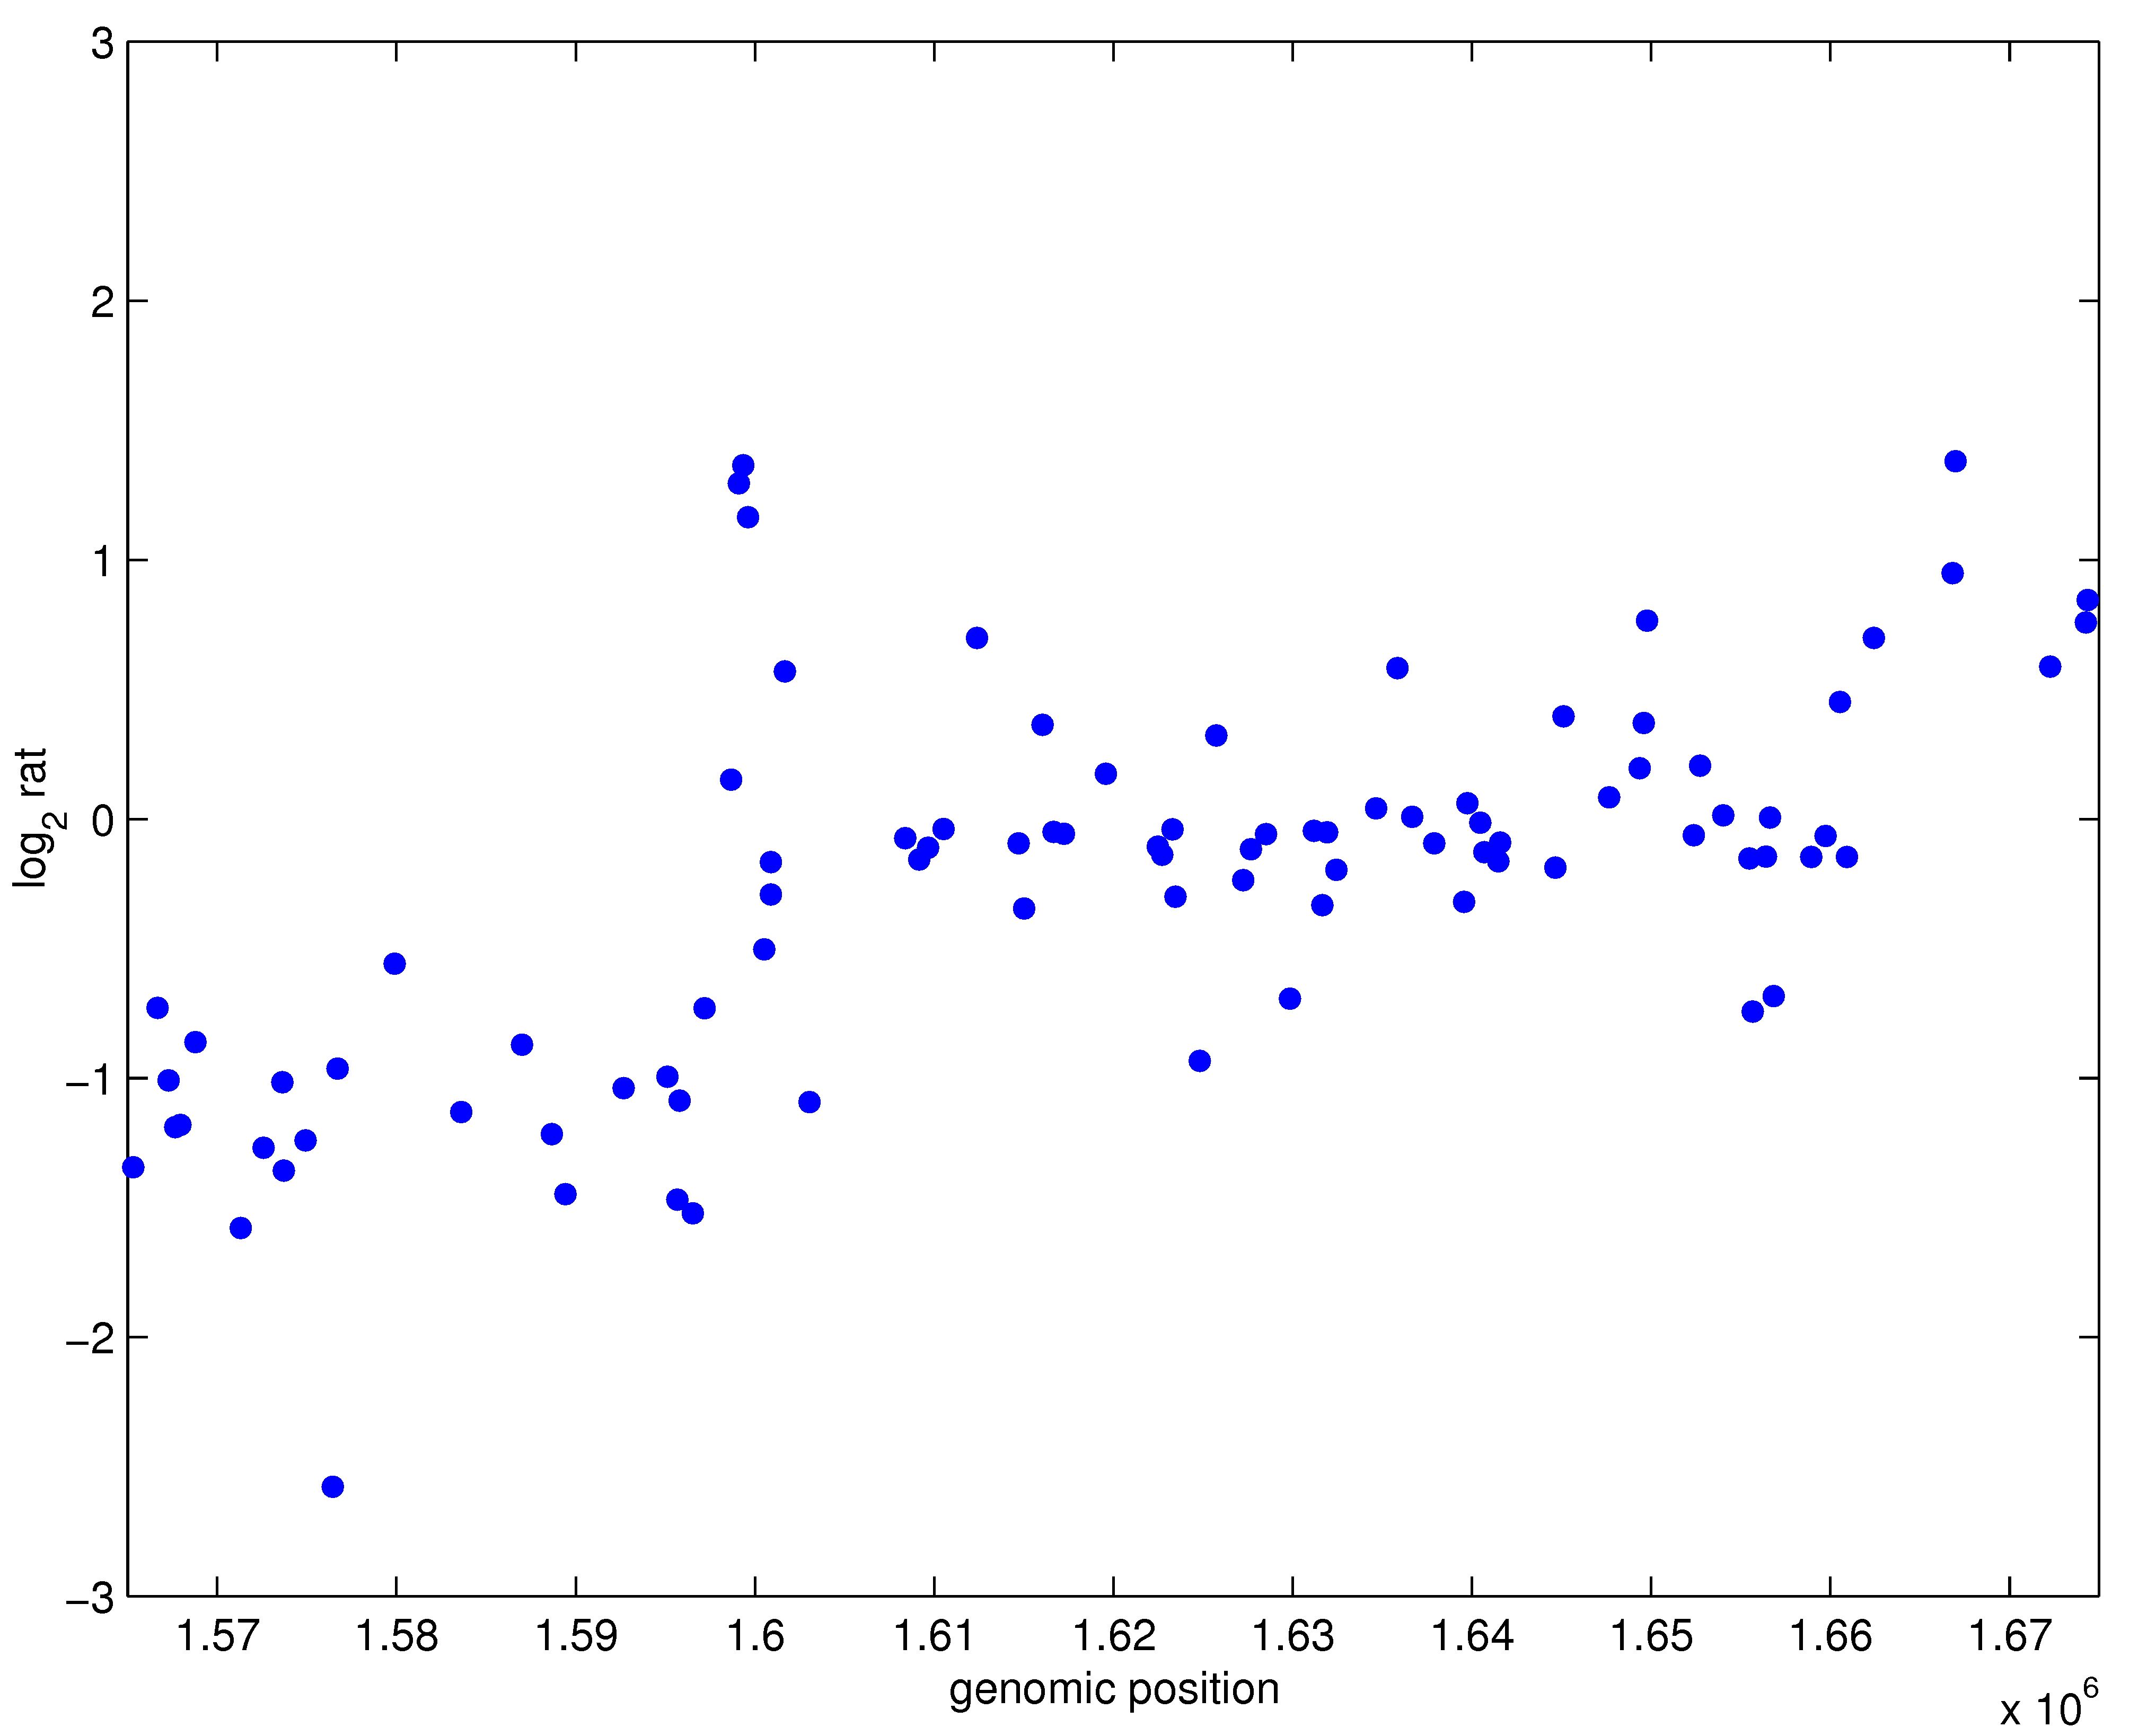
\epsfig{file = ../Figures/raw_profile_example.eps, clip=}
  %bbllx=60, bblly=196, bburx=543, bbury=586}
$$
\centerline{
  A dot on the graph 
  $
  \displaystyle{
    = \log_2 \left\{ \frac{\text{ $\sharp$ copies of BAC(t) in the test
          genome }}{\text{$\sharp$ copies of BAC(t) in the reference
          genome}}\right\}}
  $
}

%%%%%%%%%%%%%%%%%%%%%%%%%%%%%%%%%%%%%%%%%%%%%%%%%%%%%%%%%%%%%
\newpage
\subsection{Interpretation of a CGH profile }
%%%%%%%%%%%%%%%%%%%%%%%%%%%%%%%%%%%%%%%%%%%%%%%%%%%%%%%%%%%%%

$$
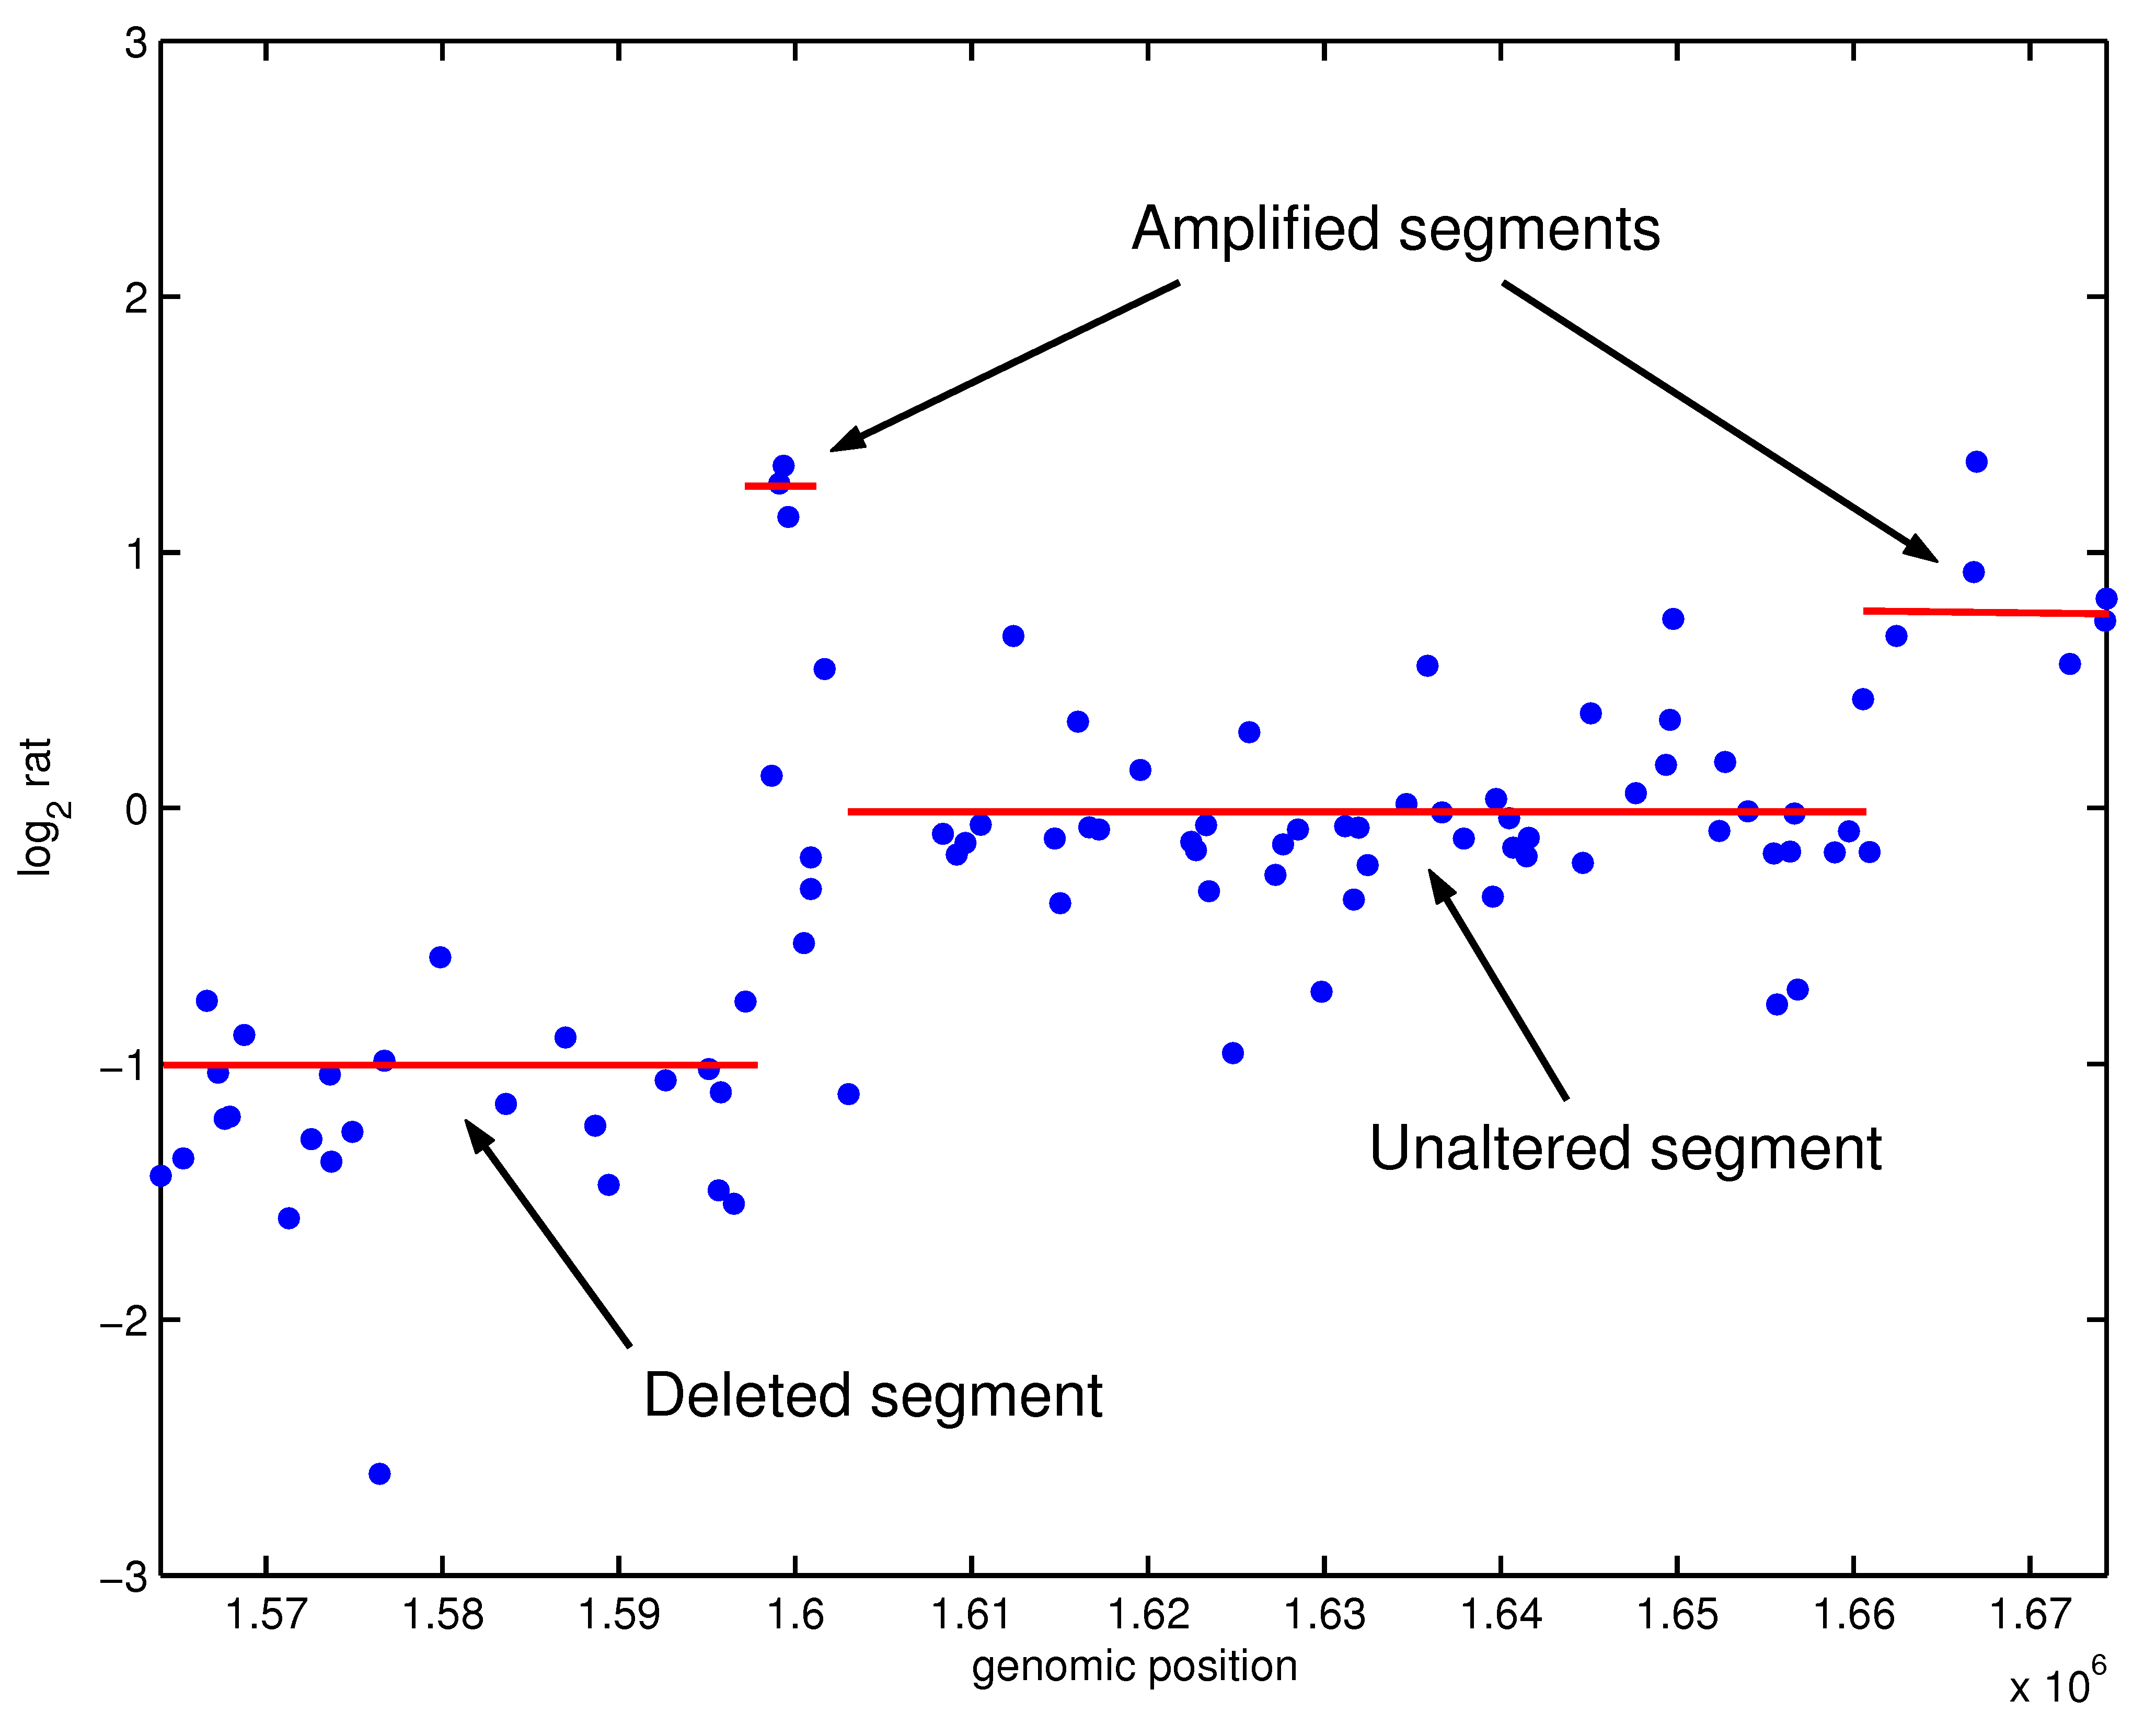
\epsfig{file = ../Figures/profile_example.eps, clip=,
  bbllx=60, bblly=196, bburx=543, bbury=586}
$$

%%%%%%%%%%%%%%%%%%%%%%%%%%%%%%%%%%%%%%%%%%%%%%%%%%%%%%%%%
\newpage
\section{Model = What we have in mind}
%%%%%%%%%%%%%%%%%%%%%%%%%%%%%%%%%%%%%%%%%%%%%%%%%%%%%%%%%%

\begin{itemize}
\item At position $t$, there exists a 'true' log-ratio $\lambda_t$,
  which depends on the relative copy number.
\item \vspace{-0.5cm} The value of the true log-ratio $\lambda_t$ is
  affected by abrupt changes:
                                %\vspace{-0.5cm}
  $$
  \epsfig{file = ../Figures/FigSeg_Intro.eps, clip=, bbllx=90,
    bblly=300, bburx=540, bbury=400, scale = 1.2}
  $$
  Position \paragraph{$t_1$, $t_2$, ..} are called {\sl
    breakpoints}. \paragraph{$\mu_k$} is the true log-ratio in segment
  \paragraph{$I_k$}.
\item \vspace{-0.5cm} The observed signal $Y_t$ is noisy:
  $$
  Y_t = \lambda_t + E_t.
  $$
%   where $\lambda_t$ is the true log-ratio and $E_t$ is a noise
%   (typically, $E_t \sim \Ncal(0, \sigma^2)$).
\end{itemize}
\vspace{-0.5cm} Breakpoints detection aims at studying the
\textblue{spatial structure of the signal}.

%%%%%%%%%%%%%%%%%%%%%%%%%%%%%%%%%%%%%%%%%%%%%%%%%%%%%%%%%%
\newpage
\subsection{Statistical model} 
%%%%%%%%%%%%%%%%%%%%%%%%%%%%%%%%%%%%%%%%%%%%%%%%%%%%%%%%%%
\vspace{-0.5cm}\begin{itemize}
\item The breakpoints define a partition of the data into $K$
  segments of size $n_k$:
  $$
  I_k=\{t, t \in ]t_{k-1},t_k]\}.
%   \qquad
%   Y^k=\{Y_t, t \in I_k\}.
  $$
\item \vspace{-0.5cm} Suppose that those parameters are constant
  between two changes: 
  $$
  \mbox{if position $t$ is in segment $I_k$,} \qquad Y_t = \mu_k +
  E_t \sim \Ncal(\mu_k,\sigma_{(k)}^2).
  $$
\item \vspace{-0.5cm} The parameters of this model are: 
  $$
  T  =  (t_1, ..., t_{K-1}),
  \qquad
  \Theta  = (\theta_1,\hdots,\theta_K), \quad \theta_k=(\mu_k,\sigma_{(k)}^2).
  $$
\item \vspace{-0.5cm} The model can rewritten as a \emphase{regression
    model}:
  $$
  \Ybf = \Tbf \mubf + \Ebf
  $$
  \begin{tabular}{crcl}
    where & $\Tbf$ & = & \emphase{unknown} $n \times K$ segmentation
    matrix $(Y_{tk} = \Ibb\{i \in I_k\}$), \\
    & $\mubf$ & = & vector of the $K$ segment means.
  \end{tabular}
\end{itemize}

%%%%%%%%%%%%%%%%%%%%%%%%%%%%%%%%%%%%%%%%%%%%%%%%%%%%%%%%%%
\newpage
\subsection{Estimating the parameters}
%%%%%%%%%%%%%%%%%%%%%%%%%%%%%%%%%%%%%%%%%%%%%%%%%%%%%%%%%%

\paragraph{Log-Likelihood} (with a constant variance $\sigma^2$):
\begin{eqnarray*}
2 \Lcal_K(T, \Theta) & = & 2 \sum_{k=1}^K \log \phi(\{Y_t\}_{t \in I_k};
\theta_k) \quad = \quad 2 \sum_{k=1}^K \sum_{t \in I_k}\log \phi(Y_t; \theta_k) \\
& = & -n \log \sigma^2 - \frac1{\sigma^2} \emphase{\sum_{k=1}^K \sum_{t \in
  I_k} (Y_t - \mu_k)^2} + \mbox{cst}. 
\end{eqnarray*}

\begin{itemize}
\item Because the data are supposed to be independent, the
log-likelihood is a sum over all the segments (\emphase{additive
contrast}).
\item Because the data are supposed to be Gaussian, maximum likelihood
  estimation is equivalent to \emphase{least squares} fitting.
\item When the segments are known, estimation is straightforward:
  $\widehat{\mu}_k = \frac1{n_k} \sum_{t \in I_k} Y_t$.
\end{itemize}

% %%%%%%%%%%%%%%%%%%%%%%%%%%%%%%%%%%%%%%%%%%%%%%%%%%%%%%%%%%
% \newpage
% \paragraph{When the breakpoints are known.}
% Since we are in a Gaussian framework, maximum likelihood is equivalent
% to least squares estimate, so we get for the mean:
% $$
% \widehat{\mu}_k = \frac1{n_k} \sum_{t \in I_k} Y_t
% $$
% and for the variance,
% \begin{itemize}
% \item if it is supposed to be constant along the whole chromosome:
%   $$
%   \widehat{\sigma}^2 =  \frac1{n} \sum_{k=1}^K \sum_{t \in I_k} (Y_t -
%   \widehat{\mu}_k)^2 
%   $$
% \item if it is supposed to be specific to each segment:
%   $$
%   \widehat{\sigma}^2_k = \frac1{n_k} \sum_{t \in I_k} (Y_t -
%   \widehat{\mu}_k)^2 
%   $$
% \end{itemize}

%%%%%%%%%%%%%%%%%%%%%%%%%%%%%%%%%%%%%%%%%%%%%%%%%%%%%%%%%%
\newpage
\subsection{How to find the breakpoints?}

When $K$ is known , we have to minimise
$$
J_k(1, n) = \sum_{k=1}^K \sum_{t \in I_k} (Y_t - \widehat{\mu}_k)^2.
$$
\begin{itemize}
\item There are $\coefbin{n-1}{K-1}$ possible choices for the
  positions of the breakpoints $t_1, t_2, \dots, t_{K-1}$: \\
  \\
  \centerline{$\Rightarrow$ Impossible to explore for large
    $n$ and $K$}
\item $\sum_{t \in I_k} (Y_t - \widehat{\mu}_k)^2$ can be viewed as
  the 'cost' of segment $I_k$, i.e. the cost of putting data
  $Y_{t_{k-1}+1}$ to $Y_{t_{k+1}}$ in a single segment.
\item The optimisation problem is actually a shortest path problem
  that can be solved thanks to \paragraph{dynamic programming}.
\end{itemize}

%%%%%%%%%%%%%%%%%%%%%%%%%%%%%%%%%%%%%%%%%%%%%%%%%%%%%%%%%%
\newpage
\subsection{Dynamic programming.} Based on Bellmann's optimality
principle: \\
\\
\centerline{\framebox{\emphase{\sl Sub-paths of the optimal path are themselves
    optimal.}}} 

\bigskip\bigskip
\paragraph{Initialisation:} For $0 \leq i < j \leq n$:
$$
J_1(i, j) = \sum_{t=i+1}^j (Y_t - \widehat{\mu})^2.
$$

\paragraph{Step $k$:} For $2 \leq k \leq K$:
$$
J_k(i, j) = \min_{i \leq h \leq j} \left[J_{k-1}(1, h) + J_1(h+1,
  j)\right].
$$
$J_k$ is called the \textblue{cost matrix}. 

The global optimum is given by $J_k(1, n)$.

% \paragraph{Remark:} Same principle as the Smith-Watermann algorithm
% for sequence alignment.

%%%%%%%%%%%%%%%%%%%%%%%%%%%%%%%%%%%%%%%%%%%%%%%%%%%%%%%%%%
\newpage
\subsection{Example with $R$}

\noindent
\begin{tabular}{ll}
  \begin{tabular}{p{12cm}}
    \paragraph{Cost matrix:}
    {\tt %\small
\begin{verbatim}
lmin = 2
C = matrix(Inf, n, n)
for (i in (1:(n-lmin))) 
  {
  for (j in ((i+lmin):n)) 
  {
    reg = lm(y[i:j] ~ x[i:j])
    C[i, j] = sum(reg$residuals^2)
    } 
  }
\end{verbatim}
      }
  \end{tabular}
  &
  \begin{tabular}{p{12cm}}
    \paragraph{Breakpoints:}
    {\tt %\small
\begin{verbatim}
$t.est
      [,1] [,2] [,3] [,4] [,5] 
 [1,]   40    0    0    0    0 
 [2,]   10   40    0    0    0 
 [3,]   16   30   40    0    0 
 [4,]   10   16   30   40    0 
 [5,]   10   16   24   30   40 
\end{verbatim}
      }
  \\ \\ \\ \\
  \end{tabular} 
\end{tabular}

\paragraph{Contrasts:} 
{\tt %\small
\begin{verbatim}
$J.est
 [1] 23.8693554  9.8660559  2.6290695  1.5546431  1.2213389  
\end{verbatim}
}

%%%%%%%%%%%%%%%%%%%%%%%%%%%%%%%%%%%%%%%%%%%%%%%%%%%%%%%%%%
\newpage
\subsection{One last problem: the selection of $K$}

\noindent
\begin{tabular}{cc}
  \begin{tabular}{p{11cm}}
    \begin{itemize}
    \item The contrast $J_K$ necessarily decreases when the model
      becomes more complex. 
    \item The penalty function measures this complexity: $pen(K) = $
      $K+1$ with constant variance, $2K$ with heterogeneous variance.
    \item We look for the minimum of
      $$
      J_k + \beta pen(K)
      $$
      where $\beta$ is adaptively estimated ({\sl Lavielle(2003)}).
    \end{itemize}
  \end{tabular}
  &
  \begin{tabular}{c}
    \epsfig{file = ../Figures/Select_K.ps, clip=, bbllx=146, bblly=529,
      bburx=464, bbury=777, width=12cm, height=12cm} 
  \end{tabular}
\end{tabular}

%%%%%%%%%%%%%%%%%%%%%%%%%%%%%%%%%%%%%%%%%%%%%%%%%%%%%%%%%%
\newpage
\section{Example of segmentation on array CGH data}
%%%%%%%%%%%%%%%%%%%%%%%%%%%%%%%%%%%%%%%%%%%%%%%%%%%%%%%%%%

\paragraph{Are the variances $\sigma^2_k$ homogeneous?} BT474 cell
line, chromosome 9: 
$$
\begin{tabular}{cc}
  Homogeneous variances & Heterogeneous variances \\
  \multicolumn{2}{c}{$K=4$ segments} \\
  \epsfig{file = ../Figures/bt474_c9_seg_homo_K4.eps, clip=, scale=0.7} &
  \epsfig{file = ../Figures/bt474_c9_seg_hetero_K4.eps, clip=, scale=0.7} \\
\end{tabular}
$$

%%%%%%%%%%%%%%%%%%%%%%%%%%%%%%%%%%%%%%%%%%%%%%%%%%%%%%%%%%
\newpage
\paragraph{Adaptive choice of the number of segments.} BT474 cell
line, chromosome 1:
$$
\begin{tabular}{cc}
  Homogeneous variances & Heterogeneous variances \\
  $\widehat{K} = 10$  segments & $\widehat{K} = 2$ segments \\
  \epsfig{file = ../Figures/bt474_c1_seg_homo_K10.eps, clip=, scale=0.7} &
  \epsfig{file = ../Figures/bt474_c1_seg_hetero_K2.eps, clip=, scale=0.7} \\
\end{tabular}
$$
Homogeneous variances result in smaller segments. \refer{Picard \& al, 05}

%%%%%%%%%%%%%%%%%%%%%%%%%%%%%%%%%%%%%%%%%%%%%%%%%%%%%%%%%%
\newpage
\subsection{Comparative study} 

\paragraph{Lai \& al. (Bioinformatics, 05).} On both synthetic and
real data (GBM brain tumor data), the methods performs well.
$$
%\epsfig{file = ../Figures/LPJ05-Fig1.eps, clip=, scale=1.2}
%\epsfig{file = ../Figures/LPJ05-Fig3.eps, clip=, scale=1.2}
\epsfig{file = ../Figures/LPJ05-Fig4.eps, clip=, scale=1.2}
$$

% %%%%%%%%%%%%%%%%%%%%%%%%%%%%%%%%%%%%%%%%%%%%%%%%%%%%%%%%%
% \newpage
% \paragraph{ROC curves.} The sensitivity decreases for small segments
% when  signal-to-noise ratio (SNR) is small.
% $$
% \epsfig{file = ../Figures/LPJ05-Fig2.eps, clip=, scale=1.2}
% $$

%%%%%%%%%%%%%%%%%%%%%%%%%%%%%%%%%%%%%%%%%%%%%%%%%%%%%%%%%%
%%%%%%%%%%%%%%%%%%%%%%%%%%%%%%%%%%%%%%%%%%%%%%%%%%%%%%%%%%%%%
\newpage
\chapter{Breakpoint detection with covariates}
%%%%%%%%%%%%%%%%%%%%%%%%%%%%%%%%%%%%%%%%%%%%%%%%%%%%%%%%%%%%%
%%%%%%%%%%%%%%%%%%%%%%%%%%%%%%%%%%%%%%%%%%%%%%%%%%%%%%%%%%
 
%%%%%%%%%%%%%%%%%%%%%%%%%%%%%%%%%%%%%%%%%%%%%%%%%%%%%%%%%%%%%
%%%%%%%%%%%%%%%%%%%%%%%%%%%%%%%%%%%%%%%%%%%%%%%%%%%%%%%%%%%%%
\bigskip\bigskip
\section{Harvest data}
%%%%%%%%%%%%%%%%%%%%%%%%%%%%%%%%%%%%%%%%%%%%%%%%%%%%%%%%%%%%%
%%%%%%%%%%%%%%%%%%%%%%%%%%%%%%%%%%%%%%%%%%%%%%%%%%%%%%%%%%%%%
\vspace{-1.5cm}
$$
\begin{tabular}{lc}
  \begin{tabular}{p{10cm}}
    Data = Harvest dates and temperatures in Ouges (Burgundy)
    since 1882. \refer{Chuine, 04} \\ \\ \\
    A breakpoint is detected in \emphase{both series in 1986}. \\ \\ \\
    Is the 1986 breakpoint observed in harvest data caused by the
    corresponding rupture in the temperatures,
  \end{tabular}
  &  
  \begin{tabular}{c}
    {Harvest time} \\
    \epsfig{file=../Figures/Ouges_vendanges_seg_homo_hetero.ps, 
      bbllx=120, bblly=460, bburx=480, bbury=580, clip=, width=14cm,
      height=5.5cm} \\ 
    \\
    {Mean summer temperature} \\ 
    \epsfig{file=../Figures/Ouges_temp_seg_homo_hetero.ps,
      bbllx=120, bblly=460, bburx=480, bbury=580, clip=, width=14cm,
      height=5.5cm}  
  \end{tabular}
\end{tabular}
$$

%%%%%%%%%%%%%%%%%%%%%%%%%%%%%%%%%%%%%%%%%%%%%%%%%%%%%%%%%%%%%
\newpage
\section{Regression / segmentation model}
%%%%%%%%%%%%%%%%%%%%%%%%%%%%%%%%%%%%%%%%%%%%%%%%%%%%%%%%%%%%%

\hspace{-1.8cm} \begin{tabular}{lrcl}
  Denote & $Y_t$ & = & harvest date at year $t$, \\
  & $x_t$ & = & temperature at year $t$, \\
  & $I_k$  & = & $k$-th segment ($I_k=\{t, t \in ]t_{k-1},t_k]\}$).
\end{tabular} \\ \\ \\
The model is, for $t \in I_k$,
$$
Y_t = \underset{\mbox{regression}}{\underbrace{\emphase{b x_t}}} 
+ \underset{\mbox{segmentation}}{\underbrace{\emphase{\mu_k}}} + E_t
$$

\paragraph{Matrix form.} The model can be written as
$$
\Ybf + \Xbf \thetabf + \Tbf \mubf + \Ebf
$$
  \begin{tabular}{crcl}
    where & $\Xbf$ & = & known matrix of regressors (vector of
    temperatures), \\ 
    & $\thetabf$ & = & vector of regression coefficients 
    ($\thetabf = [b]$), \\
    & $\Tbf$ & = & \emphase{unknown} segmentation
    matrix $(Y_{tk} = \Ibb\{i \in I_k\}$), \\
    & $\mubf$ & = & vector of segment means. 
  \end{tabular}

%%%%%%%%%%%%%%%%%%%%%%%%%%%%%%%%%%%%%%%%%%%%%%%%%%%%%%%%%%
\newpage
\subsection{Heuristic estimation procedure}
%%%%%%%%%%%%%%%%%%%%%%%%%%%%%%%%%%%%%%%%%%%%%%%%%%%%%%%%%%

\paragraph{Least squares criterion.} We look for
$$
\underset{b, \{I_k\}, \{\mu_k\}}{\min} \sum_k \sum_{t\in I_k} (Y_t - b
x_t - \mu_k)^2,
$$
which is \emphase{not additive}, since $b$ is common to all segments.

\paragraph{Iterative heuristic.} Set $F^0_t = Y_t$ and iterate until
convergence of $b^h, \{I^h_k\}, \{\mu^h_k\}$:
\vspace{-0.5cm} \begin{enumerate}
\item Segmentation step: 
  $$
  \underset{\emphase{\{I_k\}, \{\mu_k\}}}{\min} \sum_k \sum_{t\in
    I_k} (\emphase{F^h_t} - \mu_k)^2,   
  \qquad \longrightarrow \qquad 
  \mbox{for } t \in i^{h+1}_k: \quad G^{h+1}_t = Y_t - {\mu}^{h+1}_k;
  $$
\item \vspace{-0.5cm} Regression step: 
  $$
  \underset{\emphase{b}}{\min} \sum_k \sum_{t\in I_k}
  (\emphase{G^{h+1}_t} - b x_t)^2, 
  \qquad \longrightarrow \qquad 
  F^{h+1}_t = Y_t - {b}^{h+1} x_t. 
  $$
\end{enumerate}


%%%%%%%%%%%%%%%%%%%%%%%%%%%%%%%%%%%%%%%%%%%%%%%%%%%%%%%%%%
\newpage
\subsection{Results}
%%%%%%%%%%%%%%%%%%%%%%%%%%%%%%%%%%%%%%%%%%%%%%%%%%%%%%%%%%
When accounting for temperature, the breakpoint at $t=1986$ vanishes.

\noindent
\begin{tabular}{ccc}
  & Scatter plot + Segments & Contrast \\
  \begin{tabular}{p{5cm}} Segmentation for harvest dates \\ \\ $K = 4$
    (2, 6?) \\ \end{tabular} &
  \begin{tabular}{c} \epsfig{file=../Figures/vendanges-temp-red.ps,
      clip=, width=12cm, height=5cm, bbllx=310, bburx=585, bblly=515,
      bbury=615} \end{tabular} & 
  \begin{tabular}{c} \epsfig{file=../Figures/vendanges-temp-red.ps,
      clip=, width=6cm, height=5cm, bbllx=12, bburx=285, bblly=515,
      bbury=615}  \end{tabular}\\ 
  \begin{tabular}{p{5cm}} Segmentation for temperatures \\ \\ $K = 4$
      (2?) \\ \end{tabular} &
  \begin{tabular}{c} \epsfig{file=../Figures/vendanges-temp-red.ps,
      clip=, width=12cm, height=5cm, bbllx=310, bburx=585, bblly=368,
      bbury=468}  \end{tabular}& 
  \begin{tabular}{c} \epsfig{file=../Figures/vendanges-temp-red.ps,
      clip=, width=6cm, height=5cm, bbllx=12, bburx=285, bblly=368,
      bbury=468} \end{tabular} \\ 
  \begin{tabular}{p{5cm}} Segmentation / regression for harvest dates
      \\ \\ $K = 3$ (1?) \\ \end{tabular} &  
  \begin{tabular}{c} \epsfig{file=../Figures/vendanges-temp-red.ps,
      clip=, width=12cm, height=5cm, bbllx=310, bburx=585, bblly=220,
      bbury=320} \end{tabular} & 
  \begin{tabular}{c} \epsfig{file=../Figures/vendanges-temp-red.ps,
      clip=, width=6cm, height=5cm, bbllx=12, bburx=285, bblly=220,
      bbury=320} \end{tabular} \\ 
\end{tabular}

%%%%%%%%%%%%%%%%%%%%%%%%%%%%%%%%%%%%%%%%%%%%%%%%%%%%%%%%%%
%%%%%%%%%%%%%%%%%%%%%%%%%%%%%%%%%%%%%%%%%%%%%%%%%%%%%%%%%%%%%
\newpage
\chapter{Multiple segmentation}
%%%%%%%%%%%%%%%%%%%%%%%%%%%%%%%%%%%%%%%%%%%%%%%%%%%%%%%%%%%%%
%%%%%%%%%%%%%%%%%%%%%%%%%%%%%%%%%%%%%%%%%%%%%%%%%%%%%%%%%%

%%%%%%%%%%%%%%%%%%%%%%%%%%%%%%%%%%%%%%%%%%%%%%%%%%%%%%%%%%
\bigskip\bigskip
\section{Examples}
%%%%%%%%%%%%%%%%%%%%%%%%%%%%%%%%%%%%%%%%%%%%%%%%%%%%%%%%%%

\subsection{Breakpoints in temperature series}

Consider the temperatures series $\{Y_{i t}\}$ in several French
cities ($i = 1..m$), we look for \emphase{common breakpoints} in
the climate slope $b$ accounting for a (random) \emphase{city effect
$U_i$}:
$$
t\in I_k \quad \Rightarrow \quad
Y_{i t} = \mu + U_i + b_k t + E_{i t}
$$
where $\{U_i\}$ are i.i.d. $\Ncal(0, \gamma^2)$ and $\{E_{i
  t}\}$ are i.i.d. $\Ncal(0, \sigma^2)$.

\bigskip
This model induces a correlation between all temperatures collected in
the same city:
$$
\Cov(Y_{i t}, Y_{i, t'}) = \gamma^2
\qquad \Rightarrow \qquad
\Corr(Y_{i t}, Y_{i, t'}) = \frac{\gamma^2}{\gamma^2 + \sigma^2}.
$$


%%%%%%%%%%%%%%%%%%%%%%%%%%%%%%%%%%%%%%%%%%%%%%%%%%%%%%%%%%%%%
\newpage
\subsection{Chromosomal aberrations in a set of patients}

\hspace{-2cm}
\begin{tabular}{cc}
  \begin{tabular}{p{12cm}}
    Consider the CGH profiles $\{Y_{i t}\}$ of a set of patients ($i
    = 1..m$), we look for \emphase{individual breakpoints} accounting for
    a (random) \emphase{probe effect $U_t$}:
    $$
    t\in I_{i k} \quad \Rightarrow \quad
    Y_{i t} = \mu_{i k} + U_t + E_{i t}.
    $$
    $U_t$ accounts for different probe affinities that \emphase{may
      alter all the profiles} at the same position. \\ \\
    The random term induces a correlation between all these
    measurements. 
  \end{tabular}
  &
  \begin{tabular}{l}
    \epsfig{file = ../Figures/nakao-mat.txt-MixSeg.eps, width=11cm,
    height=14cm, bbllx=90, bblly=220, bburx=380, bbury=590, clip=}
  \end{tabular}
\end{tabular}


%%%%%%%%%%%%%%%%%%%%%%%%%%%%%%%%%%%%%%%%%%%%%%%%%%%%%%%%%%
\newpage
\section{Mixed linear model with breakpoints}
%%%%%%%%%%%%%%%%%%%%%%%%%%%%%%%%%%%%%%%%%%%%%%%%%%%%%%%%%%

The general formulation of the model is 
$$
\Ybf = \Tbf \mubf + \Zbf \Ubf + \Ebf
$$
where 
\begin{description}
\item[$\Ybf$:] \vspace{-0.5cm} profiles, 
\item[$\Tbf$] \vspace{-0.5cm} segments
  (\emphase{unknown $\rightarrow$ to estimate}),
\item[$\mubf$] \vspace{-0.5cm} mean signal in each
  segment (\emphase{unknown $\rightarrow$ to estimate}),
\item[$\Zbf$] \vspace{-0.5cm} design matrix of the random effect,
\item[$\Ubf$] \vspace{-0.5cm} vector of random effect
  (\emphase{unobserved}): $\Ubf \sim \Ncal(\Obf, \Gbf)$
  (\emphase{$\Gbf$ unknown $\rightarrow$ to estimate}),
\item[$\Ebf$] \vspace{-0.5cm} residual (unobserved): $\Ubf \sim
  \Ncal(\Obf, \Rbf)$ (\emphase{$\Rbf$ diagonal, unknown $\rightarrow$
    to estimate}).
\end{description}

%%%%%%%%%%%%%%%%%%%%%%%%%%%%%%%%%%%%%%%%%%%%%%%%%%%%%%%%%%
\newpage
\subsection{Estimation of the parameters}
%%%%%%%%%%%%%%%%%%%%%%%%%%%%%%%%%%%%%%%%%%%%%%%%%%%%%%%%%%

\paragraph{Direct maximisation of the likelihood.}
The marginal distribution of $\Ybf$ is
$$
\Ybf \sim \Ncal(\Xbf \thetabf + \Tbf \mubf, \Vbf), \qquad \mbox{where
  } \Vbf = \Zbf \Gbf \Zbf' + \Rbf.
$$
Because, $\Vbf$ is not diagonal, the direct maximisation of the
observed log-likelihood $\Lcal(\Ybf)$ leads to the minimisation of a
non additive contrast.

\centerline{Dynamic programming \emphase{can not be used} to estimate
  $\Tbf$ and $\mubf$}
\bigskip

\paragraph{E-M strategy.}
Its conditional distribution given $\Ubf$ is
$$
(\Ybf \; | \; \Ubf) \sim \Ncal(\Xbf \thetabf + \Tbf \mubf + \Zbf
\Ubf, \Rbf).
$$
In the E-M algorithm ({\sl Foulley, lecture notes}), the unobserved
effect $\Ubf$ is predicted, so we have to maximise $\Lcal(\Ybf \;| \;
\Ubf)$, which involves an additive
contrast since $\Rbf$ is diagonal. 

\centerline{\emphase{Dynamic programming can be used to estimate
    $\Tbf$ and $\mubf$}}


%%%%%%%%%%%%%%%%%%%%%%%%%%%%%%%%%%%%%%%%%%%%%%%%%%%%%%%%%%
\newpage
\subsection{A DP-EM algorithm} 

\paragraph{E step.} Calculate the conditional moments of the random
effect given the data:
$$
\widehat{\Esp}(\Ubf|\Ybf), \qquad \widehat{\Var}(\Ubf|\Ybf).
$$
\paragraph{M step.} Denoting $\widehat{\Ubf} = 
\widehat{\Esp}(\Ubf|\Ybf)$ , perform the segmentation as follows:
$$
\widehat{\Tbf \mubf} = \arg\min_{\Tbf\mubf} \|\Ybf -
{\Tbf\mubf}-\Zbf \widehat{\Ubf}\|^2.
$$
A \emphase{two-stage dynamic programming} is required to
  achieve this step for numerous patients. \refer{Picard et al.}{?}

\bigskip\bigskip
\paragraph{{\tt Segclust} package.}

{\tt http://cran.r-project.org/web/packages/segclust/index.html}

%%%%%%%%%%%%%%%%%%%%%%%%%%%%%%%%%%%%%%%%%%%%%%%%%%%%%%%%%%
\newpage
\section{Applications}
%%%%%%%%%%%%%%%%%%%%%%%%%%%%%%%%%%%%%%%%%%%%%%%%%%%%%%%%%%

\subsection{Breakpoints in temperature series}

\noindent\begin{tabular}{cc}
  \begin{tabular}{p{10cm}}
    \paragraph{Data.} For several locations ($m = 25$), we measure the
    minimal daily temperature, averaged for each year from 1957 to
    2004. (Source: Meteo France). \\
    \\
    \paragraph{Model.} $t\in I_k$ \\ 
    $\Rightarrow Y_{i t} = \mu + U_i + b_k t + E_{i t}.$ \\
    \\
    \paragraph{Estimates.} \\
    $\widehat{b}_1 = 1.8\:10^{-3}$, \\
    $\widehat{b}_2 = 2.5\;10^{-2}$, \\
    $\widehat{\gamma} = 2.0, \quad \widehat{\sigma} = 0.51$. \\
    \\
  \end{tabular}
  &
  \begin{tabular}{c}
    \epsfig{file = ../Figures/SeglinregFloraison.eps, clip=,
    width=15cm, height=12cm}
  \end{tabular}
\end{tabular}

%%%%%%%%%%%%%%%%%%%%%%%%%%%%%%%%%%%%%%%%%%%%%%%%%%%%%%%%%%
\newpage
\subsection{CGH profile: Bladder cancer data}
%%%%%%%%%%%%%%%%%%%%%%%%%%%%%%%%%%%%%%%%%%%%%%%%%%%%%%%%%%

\noindent
\begin{tabular}{cc}
  \begin{tabular}{p{10cm}}
    \paragraph{Global analysis  (Inst. Curie, F. Radvanyi)} \\ \\
    We find a \emphase{large positive random effect} $U_t$ has at position
    87. \\ \\
    $\rightarrow$ \emphase{Poor probe affinity}? \\
    $\rightarrow$ \emphase{Wrong annotation}? \\
    $\rightarrow$ \emphase{Polymorphism}?
  \end{tabular}
  &
  \begin{tabular}{c}
    \epsfig{file= ../FIGURES/Random_Effect.ps, clip, width=7cm,
    height=12cm, angle=270}
  %, bbllx=100, bblly=60, bburx=510, bbury=780}
  \end{tabular} \\
  \begin{tabular}{p{10cm}}
    The mean profile of the whole set of patients can be corrected
    from the probe effect: \\
    (${\bf \cdots}$) mean of raw profiles, \\
    (${\bf \circ}$) mean of corrected profiles
  \end{tabular}
  &
  \begin{tabular}{c}
    \epsfig{file= ../FIGURES/Graphe_Profils_Moyens_Segmentes.ps, clip,
    width=7cm, height=12cm, angle=270}
  \end{tabular}
\end{tabular}

%%%%%%%%%%%%%%%%%%%%%%%%%%%%%%%%%%%%%%%%%%%%%%%%%%%%%%%%%%
\newpage
\noindent
\begin{tabular}{cc}
  \begin{tabular}{p{10cm}}
    \paragraph{Individual profiles.}
    The random effect has an influence on the segmentation. \\
    \begin{itemize}
    \item Breakpoints around position 86 are detected in individual
      profiles when analysed independently (\textred{--}).
    \item They vanish after correction of the probe effect vanish
      ({\bf --}).
    \end{itemize}
  \end{tabular}
  &
  \begin{tabular}{c}
    \epsfig{file= ../FIGURES/Profils2_9_29.ps, width=12cm,
    height=16cm, clip=} 
  \end{tabular}
\end{tabular}

%%%%%%%%%%%%%%%%%%%%%%%%%%%%%%%%%%%%%%%%%%%%%%%%%%%%%%%%%%%%%%%%%%%%%%
%%%%%%%%%%%%%%%%%%%%%%%%%%%%%%%%%%%%%%%%%%%%%%%%%%%%%%%%%%%%%%%%%%%%%%
\end{document}
%%%%%%%%%%%%%%%%%%%%%%%%%%%%%%%%%%%%%%%%%%%%%%%%%%%%%%%%%%%%%%%%%%%%%%
%%%%%%%%%%%%%%%%%%%%%%%%%%%%%%%%%%%%%%%%%%%%%%%%%%%%%%%%%%%%%%%%%%%%%%
%%%%%%%%%%%%%%%%%%%%%%%%%%%%%%%%%%%%%%%%%%%%%%%%%%%%%%%%%%
